\title{Computer Architecture - CS 301} % You may change the title if you want.

\author{Rishit Saiya - 180010027, Assignment - 12}

\date{\today}

\documentclass[12pt]{article}
\usepackage{fullpage}
\usepackage{enumitem}
\usepackage{amsmath,mathtools}
\usepackage{amssymb}
\usepackage[super]{nth}
\usepackage{textcomp}
\usepackage{hyperref}
\hypersetup{
    colorlinks=true,
    linkcolor=blue,
    filecolor=magenta,      
    urlcolor=cyan,
}
\begin{document}
\maketitle

%----------------------------------------------------------------

\section{}
This is a direct application to find the CPI as mentioned in the video lecture. Figure 1 shows the formula we will be using which is given in lecture.

\begin{figure}
    \centering
    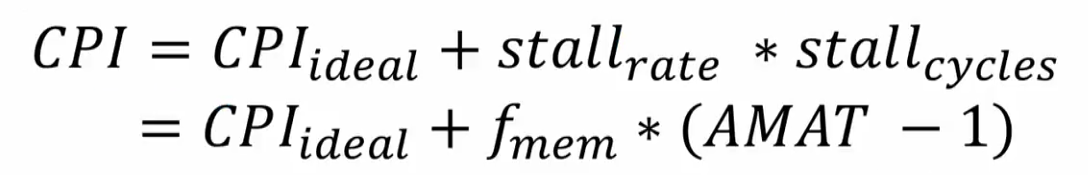
\includegraphics[width = 13cm, height = 2cm]{Assignment-12/Formula1.png}
    \caption{CPI Calculation}
    % \label{fig:my_label}
\end{figure}
In here, 1 is the $L1_{Hit \, Time}$. So, formula might change accordingly. \\
To get an overview, we will try to list down all the given values to us. They are as follows: \\
Baseline IPC = 0.8 \\
Fraction of Memory Operations = 30 \% \\
L1 Cache Hit Rate = 100 \% \\
L1 Cache Hit Time = 1 Cycle \\
L1 Data Cache Miss Rate = 5 \% \\
L2 Cache Miss Rate = 50 \% \\
L2 Cache Hit Time = 10 cycles \\
L2 Miss Penalty = 100 cycles \\

\begin{equation*}
    CPI_{ideal} = \frac{1}{IPC_{baseline}}
\end{equation*}
\begin{equation*}
    CPI_{ideal} = \frac{1}{0.8} = 10/8 = 1.25
\end{equation*}
We are given the $f_{mem}$ as follows: \\
\begin{equation*}
    f_{mem} = 30 \% = 0.3
\end{equation*}
So, we calculate the AMAT variable value. We are given in the lecture that AMAT value is as given in Figure 2. With that reference, we will calculate AMAT here.
\begin{figure}
    \centering
    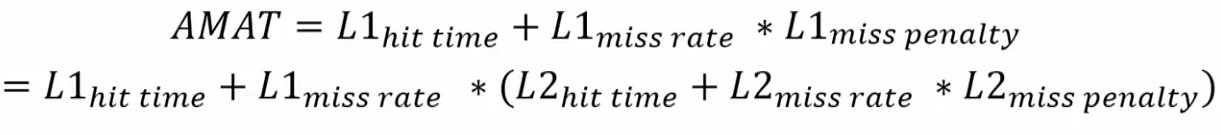
\includegraphics[width = 15cm, height = 2cm]{Assignment-12/Formula2.png}
    \caption{AMAT Calculation}
\end{figure}
\begin{equation*}
    AMAT = L1_{Hit \, Time} + L1_{Miss \, Rate} \times (L2_{Hit \, Time} + (L2_{Miss \, Rate} \times L2_{Miss \, Penalty}))
\end{equation*}
\begin{equation*}
    AMAT = 1 + 0.05 \times (10 + (0.5 \times 100)) = 4
\end{equation*}
So, finally we calculate CPI.
\begin{equation*}
    CPI = 1.25 + 0.3 \times (4 - 1) = 2.15
\end{equation*}
So, final IPC will be as follows: 
\begin{equation*}
    IPC = \frac{1}{CPI}
\end{equation*}
\begin{equation*}
    IPC = \frac{1}{2.15} = 0.4651162790
\end{equation*}
%----------------------------------------------------------------

\section{}

Before we attempt to understand the motivation of Prefetching, we need to understand the aspect and environment where it will prove to be effective. As mentioned in the lecture, we have following types of misses: 
\begin{itemize}
    \item \textbf{Compulsory Miss:}
    These misses occur when a data stream is read first time. Since it is read first time, it compulsory has to miss and hence the name. The following are some of the suggested mitigation techniques to decrease number of Compulsory Misses:
    \begin{enumerate}
        \item As mentioned in the lecture, we can increase the Block Size, in order to store more data blocks at single read and further more this will lead to usage of spatial locality. With this the number of Compulsory Misses will reduce.
        \item Another proposed mitigation is prefetching the memory locations that are to be used in the near future. This is done by generating an algorithm which can wisely and effectively guess upcoming cache locations based on usage history.
    \end{enumerate}
    \item \textbf{Conflict Miss:} 
    These misses occur when there is limited amount of associativity in a direct mapped cache or set associative cache. The following are some of the suggested mitigation techniques to decrease number of Conflict  Misses: 
    \begin{enumerate}
        \item A simple way to mitigate is to write algorithms/codes which have cache involvement. Basically, trying to put together code which is cache independent to maximum possible extent.
        \item Another way is to use a smaller fully associative cache which is meant to store the line which is thrown out of main cache so as to use immediately next time instead of fetching. This is generally called as Victim Cache.
        \item We can also increase the associativity of the cache. As mentioned in lecture, this comes with a trade off cost of high consumption of power and latency also increases resulting in slower computation time.
    \end{enumerate}
    \item \textbf{Capacity Miss:}
    These misses occur due to limited size of Cache blocks. The following are some of the suggested mitigation techniques to decrease number of Capacity  Misses: 
    \begin{enumerate}
        \item A simple fix would be straight away increase the size of Cache blocks.
        \item Another mitigation technique would be produce a novel and wise technique for prefetching in order to accommodate more such misses.
    \end{enumerate}
\end{itemize}

As clearly mentioned above, we see that two of the misses' mitigation involves Prefetching and making a novel and wise algorithm to predict the memory locations that will be used in the near future would help us to mitigate Compulsory and Capacity Misses. This would increase the overall efficiency output of the Cache and lead to increase in more hits than before. This constitutes the motivation to integrate \textbf{\textit{Prefetching}} in modern caches. \\

In the following sections, we will explain different types of Prefetching and its processes.
\begin{itemize}
    \item \textbf{Hardware Prefetching:} A hardware prefetcher is a dedicated hardware unit that predicts the memory accesses in the near future, and fetches them from the lower levels of the memory system. \\
    
    In the Figure 3, we can see the basic look of Hardware Prefetcher as mentioned in the video.
    \begin{figure}
        \centering
        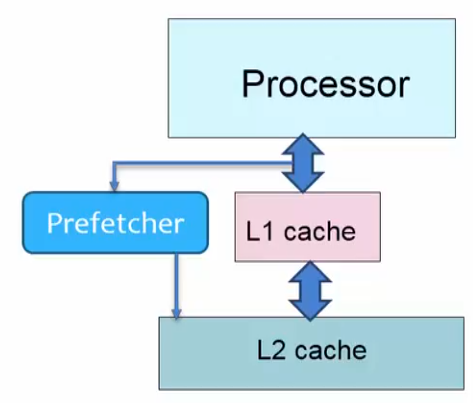
\includegraphics[width=10cm , height=8cm]{Assignment-12/Hardware_Prefetch.png}
        \caption{Hardware Prefetcher}
    \end{figure}
In here, the prefetcher checks the hits/misses at the L1 cache. Based on results from L1 cache, now it decides whether the lists of addresses are likely to be accessed in the near future or not. It then sends the data to L2 cache to get in those lines to L1 cache in a such a way that when there is a call for those data, there is a hit in L1 cache and it can easily fetch there onwards.
    \item \textbf{Software Prefetching:} A software prefetcher uses the compiler and predicts future cache misses and inserts a prefetch instruction based on the miss penalty and execution time of the instructions. \\
Below we will consider 2 different code snippets taken from the lecture to explain software Prefetching. Let us consider following Code\_Snippet-1:
\begin{verbatim}
int addAll(int data[], int vals[]) {
      int i, sum = 0;
      for (i = 0; i < N; i++) {
         sum += data[vals[i]];
      }
      return sum;
}
\end{verbatim}
Let us consider following Code\_Snippet-2:
\begin{verbatim}
int addAllP(int data[], int vals[]) {
      int i, sum = 0;
      for (i = 0; i < N; i++) {
         __builtin_prefetch(& data[vals[i + 100]]);
         sum += data[vals[i]];
      }
    return sum;
}
\end{verbatim}
Since \textit{vals} array can have discrete values and can be stored in the sequence, \textit{vals} array possess spatial locality whereas \textit{data} array doesn't has any spatial locality. In such case, we integrate the above function in Code\_Snippet-1 with \textit{\_\_builtin\_prefetch} function which helps us to prefetch the address of data which are to be accessed after such 100 iterations. This helps us to increase the Memory Fetch efficiency of cache and also to reduce the MA time.
\end{itemize}

As much as Prefetching techniques are helping us to mitigate compulsory and capacity misses, there also exists some disadvantages of using it. Some of which are as follows: 
\begin{itemize}
    \item Addition of Extra Complexity to the Code Execution
    \item Addition of Risk of displacing useful/frequently used data from the caches.
\end{itemize}
Source used: Reference Book, Video Lecture,  \href{https://en.wikipedia.org/wiki/Cache_prefetching}{Wiki Page}
%----------------------------------------------------------------
\end{document}